% easychair.tex,v 3.1 2011/12/30
%
% Select appropriate paper format in your document class as
% instructed by your conference organizers. Only withtimes
% and notimes can be used in proceedings created by EasyChair
%
% The available formats are 'letterpaper' and 'a4paper' with
% the former being the default if omitted as in the example
% below.
%
\documentclass[procedia]{easychair}
%\documentclass[debug]{easychair}
%\documentclass[verbose]{easychair}
%\documentclass[notimes]{easychair}
%\documentclass[withtimes]{easychair}
%\documentclass[a4paper]{easychair}
%\documentclass[letterpaper]{easychair}

% This provides the \BibTeX macro
\usepackage{doc}
\usepackage{makeidx}
\usepackage{multirow}
\usepackage{array}

% In order to save space or manage large tables or figures in a
% landcape-like text, you can use the rotating and pdflscape
% packages. Uncomment the desired from the below.
%
% \usepackage{rotating}
% \usepackage{pdflscape}

% If you plan on including some algorithm specification, we recommend
% the below package. Read more details on the custom options of the
% package documentation.
%
% \usepackage{algorithm2e}

% Some of our commands for this guide.
%
\newcommand{\easychair}{\textsf{gpnn}}
\newcommand{\miktex}{MiK{\TeX}}
\newcommand{\texniccenter}{{\TeX}nicCenter}
\newcommand{\makefile}{\texttt{Makefile}}
\newcommand{\latexeditor}{LEd}

\def\procediaConference{99th Conference on Topics of
  Superb Significance (COOL 2014)}

%\makeindex

%% Front Matter
%%
% Regular title as in the article class.
%
\title{A Computational Framework for Implementation of\\
       Neural Networks on Multicore Machine}

% \titlerunning{} has to be set to either the main title or its shorter
% version for the running heads. When processed by
% EasyChair, this command is mandatory: a document without \titlerunning
% will be rejected by EasyChair

\titlerunning{Parallelized Neural Networks Framework}

% Authors are joined by \and. Their affiliations are given by \inst, which indexes into the list
% defined using \institute
%
\author{
    Wenduo Wang\inst{1}%\thanks{Designed and implemented the class style}
\and
    Yi L. Murphey\inst{2}%\thanks{Masterminded EasyChair and created versions 3.0--3.4 of the class style}\\
}

% Institutes for affiliations are also joined by \and,
\institute{
  University of Michigan-Dearborn,
  Dearborn, Michigan, U.S.A\\
  \email{wenduow@umich.edu}
\and
   University of Michigan-Dearborn,
   Dearborn, Michigan, U.S.A\\
   \email{yilu@umich.edu}\\
}

%  \authorrunning{} has to be set for the shorter version of the authors' names;
% otherwise a warning will be rendered in the running heads. When processed by
% EasyChair, this command is mandatory: a document without \authorrunning
% will be rejected by EasyChair

\authorrunning{Wang and Murphey}

\begin{document}

\maketitle

\keywords{algorithm, back-propagation, neural networks, parallel computing, generic programming}

\begin{abstract}

This paper presents a computational framework, GPNN, for efficient implementation of Back-Propagation based neural network training on multithread and multicore machines. GPNN has three components, parallelization of training process, abstraction modeling of network components, and generic programming to make neural network systems to change architectural configurations.  The penalization component distributes training data to multicores to calculate errors, which are then summarized and used for weight update based on gradient descent the multithread programming to take advantage of a multicore computer architecture.  The abstraction component models input, bias, weight, and neuron all as nodes, which make the training process in a parallel computer architecture much more efficient.  The generic programming component will make a neural network system easy to change its configurations and easily transported among different operating systems or computer hardware systems.  The GPNN was applied to four different neural learning algorithms, Classic Back-Propagation (BP), Quick Propagation (QP), Resilient Propagation (RP) and Levenberg-Marquardt Algorithm (LMA), and experiments are conducted to evaluate the efficiency of these neural network algorithms implemented under the GPNN framework.

\end{abstract}

%------------------------------------------------------------------------------

\section{Introduction}

Artificial neural networks are used in wide range of research and applications over past three decades.  The network topology and propagation algorithms often vary with different application scenarios.  Researchers usually spend much effort and time struggling to try different network architectures, applying them to training data, and analyzing training results.  Many important issues, for example, over-fitting, network size, memory space need to be considered across the whole training procedure.  This may shifts researchers from their original topics to too much network reliability considerations.

Benefited from generic programming, researchers can easily configure their own neural networks or try among different configurations through a design pattern, as known as the policy pattern, which makes everything instantiable modules.  This library currently provides four types of networks, which are 1, 2, 3-hidden layer networks and recurrent network \cite{boden2001guide}, four types of weight update algorithms, classic back-propagation (BP), quick propagation (QP) \cite{fahlman1988empirical}, resilient propagation (RP) \cite{riedmiller1993direct} and Levenberg-Marquardt algorithms (LMA) \cite{hagan1994training}.  Besides these build-in learning models, researchers can connect or prune perceptron (using neuron instead of perceptron in rest of the article for convenience) and weights to customize any type of network topology.

With the increase number of cores or processors, appropriate parallelization and data partition can maximum training speed.  The GPNN library provides the interface for fast local file access using memory map and an interface for Map-Reduce application.  All of these operations and inner data flows during training are implemented on stack memory to avoid wasting time on dynamic allocation and access.  The only restriction of network size depends on the stack pre-allocation of compiler, which normally can be adjusted by compilers.

Different from previous works, for example, FANN \cite{nissen2003implementation}, OpenNN \cite{lopezopennn} and tnnlib, which take only partial advantages of generic programming, algorithm and topology diversity or parallel execution ability (see Appendix~ref{appendix:comparison}), the GPNN library possesses all of these attractive characteristics.

%------------------------------------------------------------------------------

\section{A Computational Framework for Implementing Neural Learning Algorithms on Multicore machines}
\label{section:implementation}

The proposed computational framework consists of three major components, parallelization of training process using a multithread scheme, abstraction of network components, and general programming on transfer functions, error functions and network topologies.  First we present a formal description of neural network structures and back-propagation neural learning algorithm from the perspective of software implementation.

In software implementation development, a classic neural network layer is normally modeled as a container, which holds a weight matrix, a bias node and multiple neurons.  Additionally, it specifies the propagation order of these components.  In a global view, layer can be connected with each other.

Back-Propagation is the most popular neural learning algorithm for supervised learning in multi-layered feed-forward networks as well as in many recurrent neural networks.  Most of the neural networks have a unique forward path.

\begin{gather}
    net_j = \sum_i w_{ji} x_i \notag \\
    x_j = f_j(net_j) \notag
\end{gather}

where $x_i$ is the outputs from the neuron $i$ in previous layer, which is regarded as the inputs of neuron $j$, $w_{ji}$ is the weight from all previous neuron $i$ to neuron $j$, net is calculated as the weighted sum of all the inputs, and $x_j$ is the output after $net_j$ filtered by the transfer function $f_j$, which is also regarded as one of the input of next layer.

The backward path follows gradient descent calculated by chain rule.

\begin{equation}
    \frac{ \partial E_j }{ \partial w_{ji} } = \frac{ \partial E_j }{ \partial x_j } \cdot \frac{ \partial x_j }{ \partial net_j } \cdot \frac{ \partial net_j }{ \partial w_{ji} } = \frac{ \partial E_j }{ \partial x_j } f'_j(net_j) x_i \notag
\end{equation}

For every hidden neuron, its gradient is affected by all of its successors.  To consistently express the gradient of output nodes and hidden nodes, let

\begin{equation}
    \delta_{ji,d} = \left \{
    \begin{array}{l l}
        t_d - y_d & \quad \text{for output neuron} \\
        \sum_k {w_{kj}\delta_{kj,d} } & \quad \text{for hidden neuron}
    \end{array} \right. \notag
\end{equation}

where $k$ contributes to next layer.

\subsection{Parallelization}

According to Moore’s law, the density of circuits doubling at every new generation \cite{chu2007map}.  In the recent years, computer systems have increased number of cores to support parallel computing.  In big data applications, it is important to implement neural learning algorithms in high level of parallelization on multicore CPUs with shared memory to achieve significant increases in CPU performance.  We propose an approach of multithread implementation of batch training BP \cite{schuessler2011parallel}.  The approach is illustrated in \ref{fig:parallelization}, where it is shown in a $K$-thread parallel computing structure, where a neural network is copies $K$ times, and the training data are distributed to these $K$ threads.  The input are processed.

\begin{figure}[tb]
    \begin{centering}
        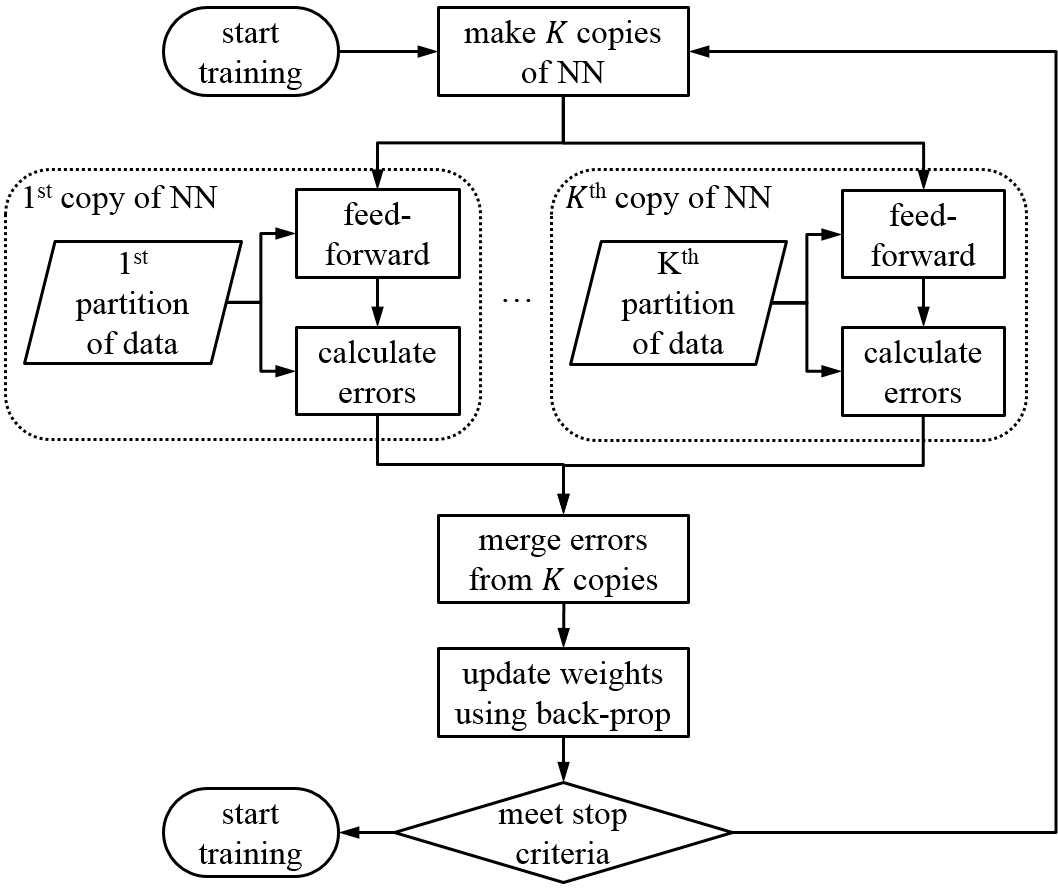
\includegraphics[scale=0.5]{../../pic/parallelization.png}
        \caption{Illustration of multithread implementation of neural learning process.}
    \label{fig:parallelization}
	\end{centering}
\end{figure}

Simultaneously along the feed-forward paths of these $K$ threads, and errors are calculated at the end of each thread.  Then the errors at all $K$ threads are combined for weight update using gradient descent (back-propagation path), which is represented as follows,

\begin{equation}
    \frac{\partial E_j}{\partial w_{ji}} = \sum_k \frac{\partial E_j^{(k)}}{\partial w_{ji}^{(k)}} \notag
\end{equation}

Weights are then all updated through back-The updated neural network is made K copies, and the same training process is repeated until user defined stop criteria are satisfied.

\subsection{Abstraction of Weight, Neuron, Bias, Input and Target}

Abstraction is a very critical and powerful concept in object-oriented programming which means to abstract as objects of similar functions to the same module.  Based on this concept, weights between neurons can be considered as similar to neurons, since a neuron has one input axon and one output axon, and a weight connecting two neurons can also be considered to have an input, which is the output axon of the preceding neuron, and the weight can be considered as its output axon that is connected to the input axon of following neuron.  The transfer function of a weight is defined as follows.

\begin{align}
    & \text{feed-forward:} & x_{ji} = f_{ji}(x_i) = w_{ji}x_i \notag \\
    & \text{back-propagation:} & \delta_j = w_{ji}\delta_{ji} \notag
\end{align}

For the same reason, an input node to a neural network can also be treated similar to a neuron, which has the equal number of output axons to the first hidden layer but no input axon.  Similarly, bias of a neuron layer can also be handled in this way.  There is no back-propagation for any of these input nodes.

\begin{align}
	& \text{feed-forward for input:} & x_i = f_0(p) = p \notag \\
	& \text{feed-forward for bias:} & x_b = f_b(1) = 1 \notag
\end{align}

where $p$ is the value of input feature, $x_i$ is the output of the input node, and the output of the bias node $x_b$ is always 1.

The output of a neuron is represented as a target node, which has one input axon connected to the output of a neural network, but no output axon, i.e., there is no feed-forward from a target node.

\begin{align}
    & \text{target node:} & \delta_j = t_j - y_j \notag
\end{align}

where $t_j$ is the target value of this output node, and $y_j$ is the network predicted value.  Target nodes are used in back-propagation process.

Based on the above discussion, input, bias, weight, neuron and target are considered as nodes in an abstraction context.  Nodes of the same type are grouped into the same abstraction layer, and these abstracted layers are connected to each other as illustrated in fig.~\ref{fig:nn_abstracted}.  A one-layer of neurons in a neural network is represented by input abs-layer (abstraction layer), bias abs-layer, weight abs-layer, neuron abs-layer and target node abs-layer.  The connection among nodes and abstracted layer are considered equivalent in the context of programming.

\begin{figure}[tb]
    \begin{centering}
        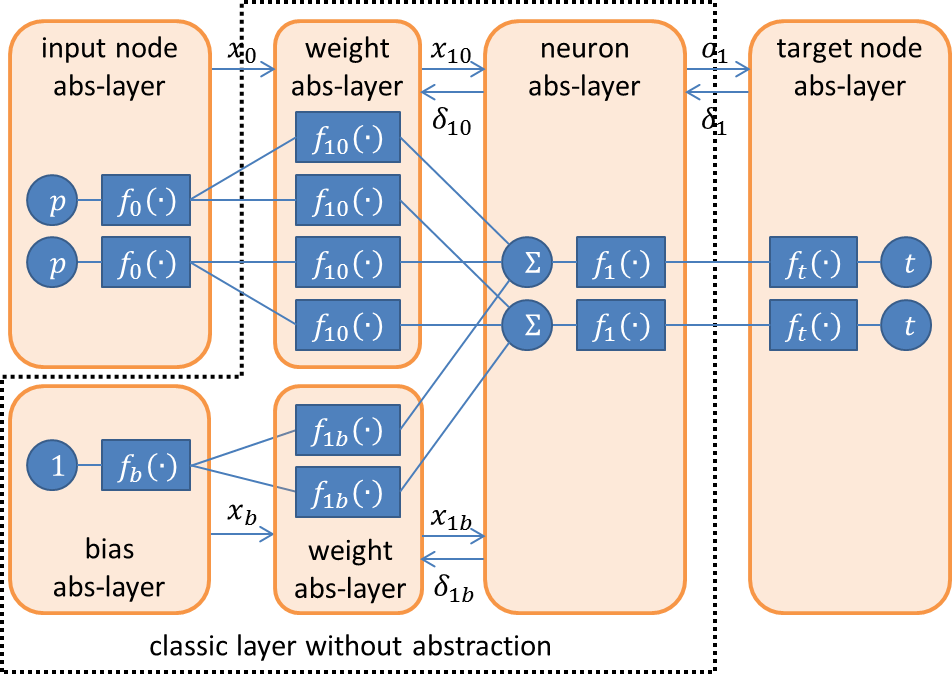
\includegraphics[scale=0.5]{../../pic/nn_abstracted.png}
        \caption{1-layer of neural network topology represented by the abstraction layers (abs-layer).  The abstracted layers inside the box in dash-line is the neural network layer.}
        \label{fig:nn_abstracted}
	\end{centering}
\end{figure}

This abstraction process provides an efficient architecture for implementing parallel computation in neural learning, since only weight abstracted layers need to be copied or shared among multiple threads as network images.  The remaining parts of the network, i.e., input nodes, biases, neurons and target nodes, can stay local without being distributed over the multicores.  Therefore the abstraction approach can reduce communicational speed and memory, which would be significant improvement over efficiency in neural learning from big data.

Current input and output of a node will be stored for each input pattern for weight update processing during the back-propagation.  Other values are prepared during feed-forward or back-propagation for intermediate calculation of critical variables, for example, $f(net)$ and $f'(net)$ shown in fig.~\ref{fig:microscopic}.

\begin{figure}[tb]
    \begin{centering}
        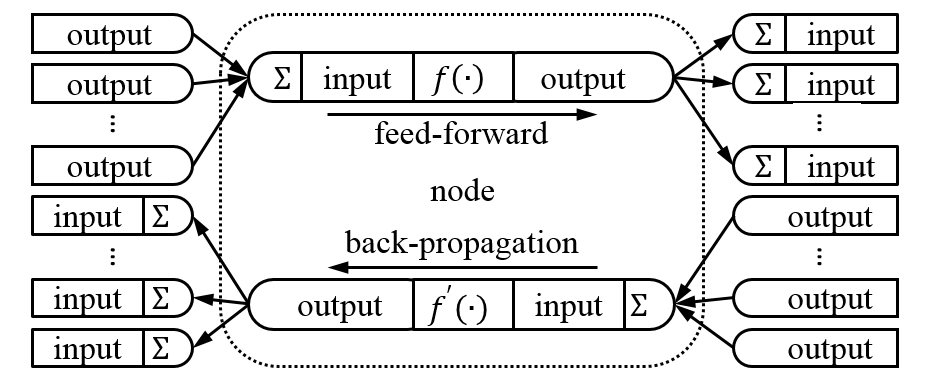
\includegraphics[scale=0.5]{../../pic/microscopic.png}
        \caption{Communication between nodes during feed-forward and back-propagation.}
        \label{fig:microscopic}
	\end{centering}
\end{figure}

\subsection{Compile-Time Generalization to Learning Algorithms, Transfer Functions, Error Functions and Network Topologies}

Generic programming is a software approach that can be used to generalize replaceable functional nodes in neural networks.   In a generic programming architecture variables can be written in terms of types to-be-specified-later  \cite{wiki:generic_programming}, and then instantiated when needed.  In neural networks, transfer functions, network topologies, and weight update functions can be type-deduced so functional call can be determined during compile time  \cite{alexandrescu2001preface}.

This compile-time generalization technique eliminates the run-time used in each loop to determine the running type of an object through looking up its virtual table.  We proposed to implement weights in compile-time generalization, since it is used in different data types including forward, backward, update and copy processes.  User can specify an appropriate update strategy of weight during programming without modifying rest part of the code.  The compiler then generate a made-to-order target file related to the developer customized behavior data types.  In addition, since the software is tailored to specific behavior data types at compiling period, this implementation greatly reduces irrelevant code, thus, reduces the software size.

Fig.~\ref{fig:run_vs_compile} illustrates the differences between run-time and compile-time implementation in a neural learning process.  In the run-time generation implementation, weight type is deduced in every epoch, which means that the processors need to spend time on deciding weight type in each loop through looking up a virtual table.  As a consequence, the accumulative time consumption from all loops is conspicuous.  If the compile-time generalization implemented, data type deduction is calculated only once at the compiling process.  Moreover, if the neural network software is required to be run multiple times for different experimental purposes, run-time generalization time on type deduction can be significant.  Contrarily, because there’s no need to compile the same neural network software again for repeated experiments, the compile-time generalization does not need extra time for data type deduction.  In summary, the time complexity for run-time generalization of weights is $O(mn)$, which can be saved if data type deduction for weights are carried out at the compiling process.

\begin{figure}[tb]
    \begin{centering}
        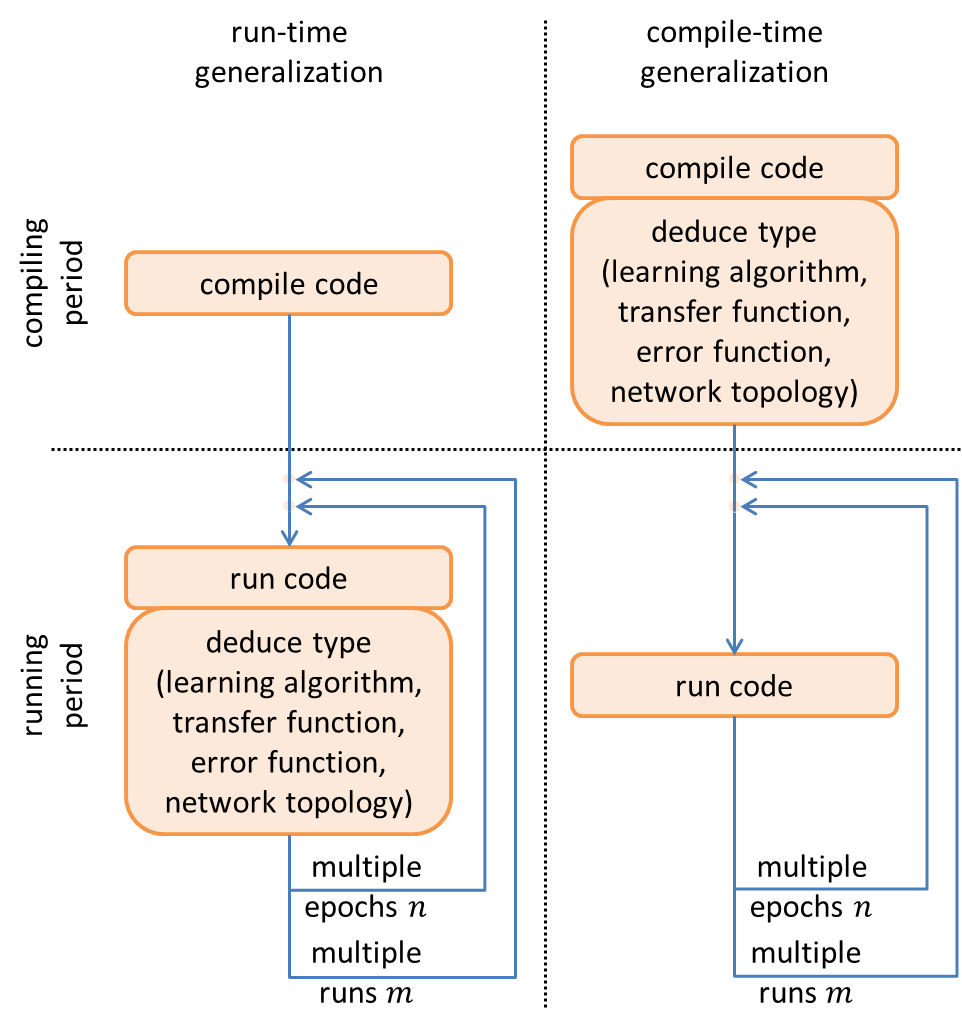
\includegraphics[scale=0.5]{../../pic/run_vs_compile.png}
        \caption{Run-time generalization versus compile-time generalization during the processes of compiling code to running code for a neural learning algorithm.  Note $n$ is epoch number and $m$ is number of experiment repeated.}
        \label{fig:run_vs_compile}
	\end{centering}
\end{figure}

In terms of design pattern, the compile-time generalization approach is as known as policy based class design \cite{alexandrescu2001policy}.  In our implementation of a library of back-propagation-based neural networks, a learning algorithm is defined as a type of update policy, a transfer function is defined as a type of transfer policy, a network topology is defined as a kind of topology policy, an error function is defined as a kind of error policy, and even the number of neurons, input, target and other training factors can be considered as individual value policies as well.

\subsection{Flexibility and Reusability of GPNN Framework}

In addition to the fast implementation of neural learning algorithms, the proposed GPNN framework also provides flexibility and reusability for neural network research.  The abstraction and compile-time generalization processes in GPNN allow researchers to build new neural networks by simply connecting or pruning nodes without re-design the most part of an existing network architecture.  For example, the following algorithms shows the steps to build a recurrent neural network without bias using LMA and log-sigmoid transfer function based on an existing biased 1-layer neural network using BP algorithm and linear transfer function.

Building a recurrent neural network:

\begin{enumerate}
    \item Detach the bias abstracted layer and the weight abstracted layer in the given neural network.
    \item Attach a neuron abstracted layer using linear transfer function, and attach a weight abstracted layer using LMA.
    \item Replace the algorithm type of the weight abstracted layer from BP to LMA, and replace the transfer function type of the neuron abstracted layer from log-sigmoid to linear.
\end{enumerate}

\begin{figure}[h]
    \begin{centering}
        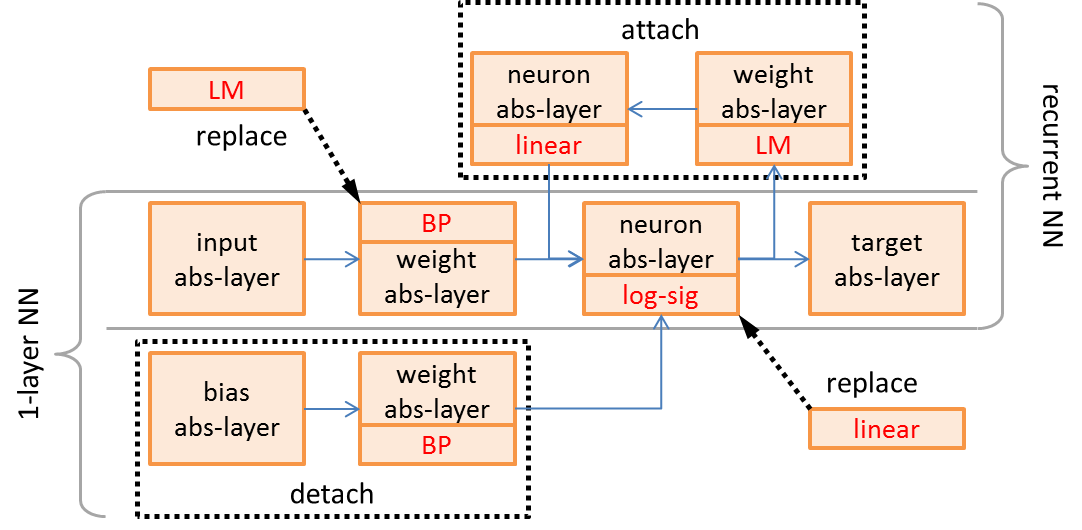
\includegraphics[scale=0.5]{../../pic/reusability.png}
        \caption{Building a recurrent neural network by modifying a 1-layer neural network.}
        \label{fig:reusability}
	\end{centering}
\end{figure}

%------------------------------------------------------------------------------

\section{Performance and Experiment Result}

We applied the proposed computational framework, GPNN, to four back-propagation based neural learning algorithms, Classic Back-Propagation (BP), Quick Propagation (QP), Resilient Propagation (RP) and Levenberg-Marquardt Algorithm (LMA).

The Quick Propagation is to take the largest steps possible to local minima without overshooting.  The QP learning algorithm is based on the assumption that the error versus weight curve can be approximated by a parabola whose arms open upward \cite{fahlman1988empirical}, which means its second derivative is approximate a line with positive slope k.  For a parabola curve, the minimum value is where its second derivative equals to 0.  QP is efficient for large training data.

The basic idea of Resilient Propagation is that every time the gradient changes its sign, it indicates that the last update was so big that the error function skipped a local minimum.  Thus, the weight update absolute value needs to be reduced by factor $ \eta ^ - $, where $ 0 < \eta ^ - < 1 $.  Contrarily, if the gradient remains the same sign as previous update, a larger step of $\theta$ can be increased by factor  $ \eta ^ + $, where $ \eta ^ + > 1 $.  The detail of the RP algorithm can be found in \cite{riedmiller1993direct}.

Levenberg-Marquardt Algorithm aims at solving non-linear least square problem.  It interpolates between the Gauss–Newton Algorithm (GNA) and the method of gradient descent. The LMA is more robust than the GNA  \cite{hagan1994training}.

We implemented these four neural learning algorithms using the Parallelization, abstraction and compiler-time generalization processes discussed in Section~\ref{section:implementation}.

In order to evaluate the performance of the proposed GPNN, we applied the following experiment data to the four neural learning algorithms implemented using GPNN. Experiment data is selected from hourly historical climate data of Ann Arbor, MI, USA downloaded from \url{www.wunderground.com} website from year 2010 to 2013, year 2010 to 2012 as training samples and year 2013 as testing samples.  So total number of training samples is 26304, total number testing samples is 8760.  Training samples are averagely distributed on each thread of which the number is determined by the configuration of each experiment.  10 input features listed in table II are input to each neural network system and neural network output is the predicted humidity value.  All input and output are normalized to zero mean ($ \mu = 0 $)and unit standard deviation ($ \sigma = 1 $).

\begin{table}[htp]
    \centering
    \caption{Features in climate dataset}
    \begin{tabular}{ c l c c }
        \hline \hline
        Usage & Feature & Valid Range & Unit \\
        \hline
        \multirow{10}{*}{input}
            & month & 1 - 12 & - \\
            & hour & 0 - 23 & - \\
            & temperature & -50 - 150 & \(^\circ\)F \\
            & dew point & -50 - 150 & \(^\circ\)F \\
            & pressure & 28 - 31 & inHg \\
            & visibility & 0 - 10 & mile \\
            & wind direction & 0 - 359 & \(^\circ\) \\
            & wind speed & 0 - 50 & mph \\
            & gust speed & 0 - 100 & mph \\
            & precipitation & 0 - 1.5 & in \\
        \hline
        target & humidity & 0 - 100 & \% \\
        \hline \hline
    \end{tabular}
    \label{table:climate}
\end{table}

All following experiments are running on a 2.3GHz quad-core 8-thread CPU with 8G RAM machine installing 64-bit operating system.

\subsection{Multithread Efficiency}

Theoretically, multiple processors and cores can support almost any number of threads running simultaneously regardless of very large system specified limit.  However, since the communication between threads is usually implemented by a pooling approach, it takes certain amount of time to synchronize all the image threads to main network thread.  Intuitively, the most efficient number of threads should be equal to the number of cores, since running time of multi-threads on the same core will add up to no less than the running time of single thread even with thread scheduling applied.

The first experiment was conducted to evaluate different number of threads applied to different number of hidden nodes while BP was used as neural learning algorithm.  Fig.~\ref{fig:thread_efficiency} show the training time for these different neural network configurations running on different number of threads.  BP algorithm is used in this experiment, and the maximum epoch is set to 2000.

\begin{figure}[tb]
    \centering
    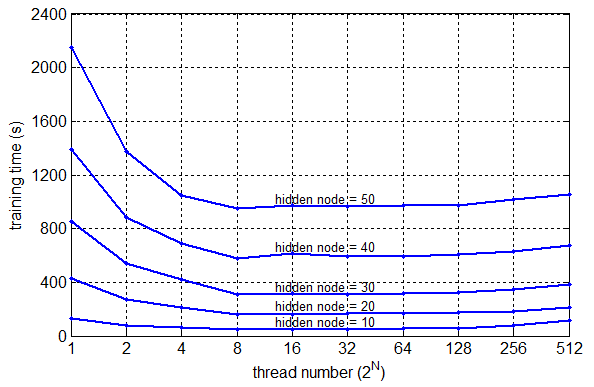
\includegraphics[scale=0.6]{../../pic/efficiency.png}
    \caption{Training time of BP for different hidden node numbers versus different numbers of threads.}
    \label{fig:thread_efficiency}
\end{figure}

The result demonstrates that the fastest thread configuration is 8 thread, which equals to the hardware concurrency of CPU in this case.  It is about 3-time ($ \frac{132}{46} \approx 2.87 $) faster than training with single thread training a 10 hidden nodes network, but it is not able to reach an ideal 8-time because of communication time cost as discussed earlier.  With the number of threads grows larger than 8, training time slightly goes up, which is due to the time cost for scheduling.

\subsection{Comparing GPNN Implementation with Conventional Implementation}

In this experiment, we evaluate the efficiency of the four neural learning algorithms implemented using GPNN and their Matlab version.  In this experiment, maximum epoch is set to 2000.  Another 10 measurements are taken independently from previous experiment, mean values are presented and standard deviation is presented as reliability.

\begin{table}[htp]
    \centering
    \caption{Training time at different thread number}
    \begin{tabular}{ l c c c c }
        \hline \hline
        Traing Time (s) & BP & QP & RP & LMA \\
        \hline
        8-thread GPNN & 56.8 & 62.4 & 69.7 & 263.9 \\
        1-thread GPNN & 176.7 & 167.9 & 192.3 & 337.7 \\
        1-thread Matlab & 649.1 & - & 678.1 & 1264.0 \\
        \hline \hline
    \end{tabular}
    \label{table:algorithm_complexity}
\end{table}

Results are shown in table~\ref{table:algorithm_complexity}.  The 8-thread implementations of BP, QP and  RP neural learning algorithms are much more computationally efficient than their respective 1-thread implementations.  LMA is more time consuming than the other three neural learning algorithms.  This is because LMA needs to calculate Hessian matrix inversion frequently even during each iteration \cite{yu2011levenberg}.  Even the 8-thread implementation of LMA does not reduce execution time much due to added time cost for communication among threads.  In the 1-thread implementation, the algorithms implemented in GPNN are more efficient than their respective functions provided by Matlab.  In comparison to their respective Mablab version, the speed up for the GPNN implemented BP is 3.6, the GPNN implemented RP is 3.5 times, and the GPNN LMA is 3.7.  Please note that the Matlab library does not have QP function.

\subsection{Algorithm Efficiency}

In reality, it is unnecessary to complete a training process up to specified maximum epoch.  Training could be terminated if certain criteria meet, for example, sum of error or gradient approximates to 0, gradient doesn’t distinctly decrease for several epochs.  Training time, converge epochs, converge error and at the termination are three measurements of efficiency among different back-propagation algorithms.  All developed algorithms participate in the comparison experiment here as configured in table~\ref{table:config_algorithm_efficiency}.  As soon as the mean absolute value of gradient is less than $10 ^ {-9}$ or not changing for 6 epochs \cite{matlab:neural_networks}, training will stop which means that error converges.  Another 10 measurements are taken independently from previous experiments and the average values are presented and standard deviation is presented as reliability.

\begin{table}[htp]
    \centering
    \caption{Converge epochs and errors of different algorithms}
    \begin{tabular}{ l c c c c }
        \hline \hline
        & BP & QP & RP & LMA \\
        \hline
        training time (s) & 3.5 & 35.1 & 28.2 & 31.1 \\
        converge epoch & 43.2 & 976.4 & 866.7 & 97.2 \\
        training error (\%) & 3.80 & 1.86 & 0.73 & 3.15 \\
        testing error (\%) & 3.66 & 1.88 & 0.76 & 33.08 \\
        \hline \hline
    \end{tabular}
    \label{table:algorithm_efficiency}
\end{table}

Results in table~\ref{table:algorithm_efficiency} shows that LMA converges faster than QP and RP, especially LMA.  However, it takes relatively more time to run because of matrix inversion time consumption discussed before.  Although RP takes more epochs to converge, its training and testing errors are distinctly smaller than others’.

According to this experiment and under the application scenario, if high accuracy is required for prediction or classification, RP algorithm is a good fit to deep dig out the local minima.  If big dataset applied and there’s no specific accuracy requirement, BP and QP algorithm could be applied.  If no more than hundreds of hidden nodes are needed, LMA could be efficient as well.

\begin{table}[htp]
    \centering
    \caption{Neural network configuration for algorithm efficiency experiment}
    \begin{tabular}{ c c c c c }
        \hline \hline
        & BP & QP & RP & LMA \\
        \hline
        thread number & 8 & 8 & 8 & 8 \\
        $\eta$ & 0.5 & 0.5 & - & - \\
        $\mu$ & - & 1.75 & - & - \\
        $\eta ^ -$ & - & - & 0.5 & - \\
        $\eta ^ +$ & - & - & 1.2 & - \\
        $\theta$ & - & - & 0.1 & - \\
        \hline \hline
    \end{tabular}
    \label{table:config_algorithm_efficiency}
\end{table}

%------------------------------------------------------------------------------

\section{Conclusion}

Based on the architecture and design pattern of this neural networks library, the author developed multiple weight update algorithms one by one after reviewing different back-propagation techniques without greatly modifying other components inside the architecture.  In terms of this, the library could be regarded as easily extendable, especially facing the circumstance that future algorithms being developed continuously.

The author created this library under the consideration of both abstraction and generalization.  It produces benefits if a network structure is not symmetric, which means user can customize the topology by pruning or branching the connections during programming.

The multithreaded architecture could easily be embedded into any kind of distributed systems by calling few functions the library provides.

The Multithreaded Neural Networks Template Library GPNN under LGPL license is available at
\url{github.com/wenduow/BeefNet}

%------------------------------------------------------------------------------

\appendix

\section{Comparison with Other Neural Networks Library}
\label{appendix:comparison}

\begin{table}[htp]
    \centering
    \caption{Neural network library characteristics}
    \begin{tabular}{ >{\centering}m{3cm} c c c c }
        \hline \hline
        Supports & FANN & OpenNN & tnnlib & GPNN \\
        \hline
        parallel computing interface & N & N & N & Y \\
        \hline 
        neural learning algorithm diversity & Y & Y & Y & Y \\
        \hline
        generic programming (strong scalability) & N & N & Y & Y \\
        \hline \hline
    \end{tabular}
    \label{table:library_compare}
\end{table}

%% References with BibTeX database:

\bibliographystyle{plain}
\bibliography{gpnn}

\end{document}

% EOF

